
\chapter{Projektion in OpenGL}

Durch die Bestimmung der Lage eines Objekts wurde ein wichtiger Teil zur Fertigstellung einer Augmented Reality Szene erreicht. Die letzte Schritt zur Darstellung eines Objekts 

\section{Transformation der extrinsischen Matrix}

\begin{figure}[!ht]
\centering
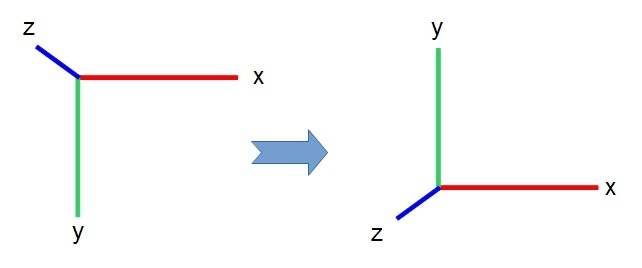
\includegraphics[scale=0.5]{images/opencv-to-opengl.jpg} 
\caption{Transformierung des Koordinatensystem von OpenCV (links) nach OpenGL (rechts).}
\label{fig:opencv-to-opengl}
\end{figure}


\section{Perspektivische Projektion}

\section{Positionierung der 3D Objekte}

\section{Konvertierung nach Core Profile}